\glsresetall

\section{Guiding longitudinal sampling in inflammatory bowel diseases 
cohorts}\label{section_ibd}

The volatile microbial signatures of \gls{cd} patients greatly hinder our 
ability to classify healthy from affected subjects using 16S rRNA profiles from 
stool. The recent work by Pascal et al. \cite{RN4208} overcomes this issue and 
other complications \cite{RN4219}, producing a decision tree that classifies 
subjects with \gls{cd}, \gls{uc}, irritable bowel syndrome and anorexia.  
Although the authors note that both subtypes of \gls{ibd}, particularly 
\gls{cd}, have increased microbial community instability, this information is 
not used as a feature to improve classifier accuracy. Could microbiome 
instability become actionable by creating a new classifier that benefits from 
repeated measurements? If so, how many samples per individual are needed to 
assess instability?

We collected daily stool samples for up to six weeks from 19 \gls{cd} subjects and 12 controls (see the analysis notebook for cohort description\footnote{\label{footlongibd}\url{https://github.com/knightlab-analyses/longitudinal-ibd}}) over 2 separate periods of 2 or 4 weeks spread over 2 and 5 months, for a total of 960 samples. We believe this is the most densely sampled longitudinal study of \gls{cd}; previous studies collected samples every 1-3 months \cite{RN1515, RN4208}. Our cohort shows decreased alpha diversity and increased stability, as previously reported in \gls{cd} and other subtypes of \gls{ibd} \cite{RN4217, RN154, RN1515, RN4208}.  We also noted that subjects who underwent resection have lower alpha diversity than other \gls{cd}-affected subjects (see analysis notebooks\textsuperscript{\ref{footlongibd}}).

A critical experimental design question for clinical studies is whether a finite budget should best be spent collecting samples from more patients, or collecting more serial samples from each patient? Therefore, we created a Random Forests \cite{RN4205} model based on per-subject aggregation of longitudinal data for alpha diversity \cite{RN4007}, beta diversity \cite{RN83} and abundances of two phylogenetic factors found to be associated with \gls{cd} in ileal biopsies \cite{RN154, RN4204} (Figure~\ref{ibd-fig1}). With one sample per subject, our model performs worse than a classifier that uses microbial relative abundances at a single time point, but when more samples per-subject are added, the classifier outperforms that approach and results previously only attained with biopsy samples \cite{RN154}. Furthermore, we replicate this observation with a different cohort (Table~\ref{ibd-table1}).

\begin{sidewaysfigure}[htbp]
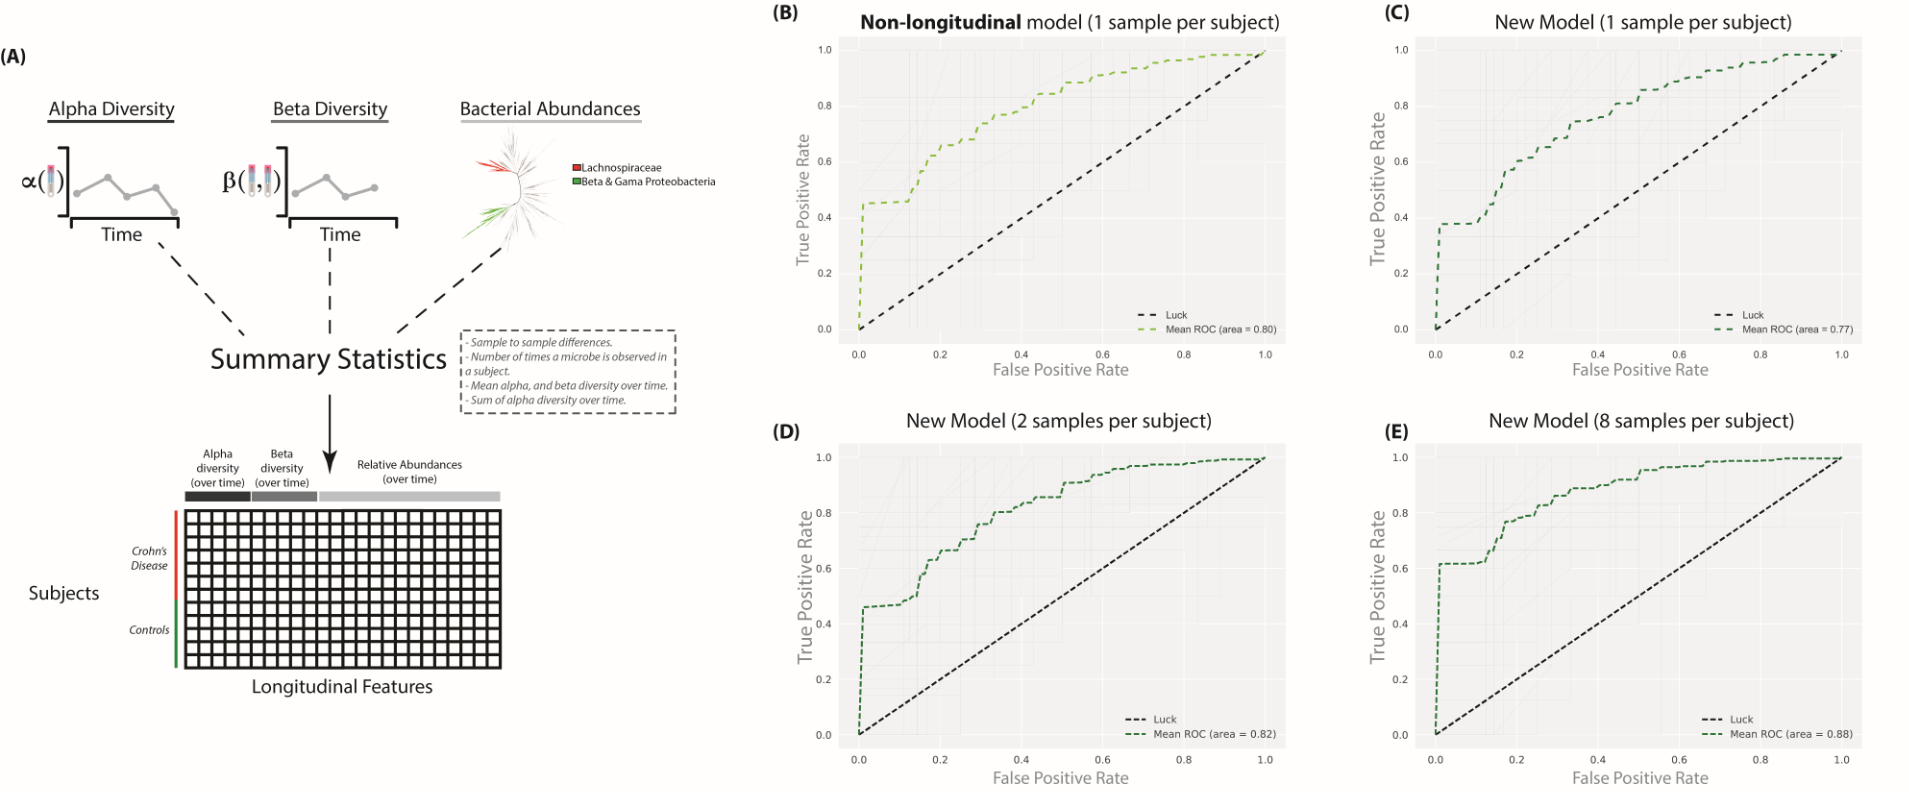
\includegraphics[width=0.95\textheight]{ibd-figures/figure-1}
\caption[Diagram for the model creation, and comparison of four receiver operating characteristic (ROC) curves.]{Diagram for the model creation, and comparison of four receiver operating characteristic (ROC) curves. (A) Diagram describing the origin for the classifying features. (B) ROC curve for a model that relies on relative abundances and one sample per subject (as used in previous publications). (C-D) ROC curve for our new model at 1, 2 and 8 samples per subject. The gray lines represent the performance at each of the 100 iterations. The dotted black diagonal line represents the performance of a classifier that guesses the labels at random.}\label{ibd-fig1}
\end{sidewaysfigure}

\begin{table}[htbp]
\centering
\caption[Performance summary of the classifier at increased samples per subject for this cohort (daily samples) and a previously published cohort.]{Performance summary of the classifier at increased samples per subject for this cohort (daily samples) and a previously published cohort. The area under the curve (AUC) summarizes the performance; closer to 1 is better, of the model trained on the different sample sizes as described by the other columns. The row marked with † represents the performance of a classifier that relies on non-longitudinal relative abundances only.}\label{ibd-table1}
\renewcommand{\arraystretch}{0.8}% Tighter
\begin{tabular*}{\textwidth}{ccccc}
\toprule
AUC &	Samples per Subject &	Controls &	Crohn's Disease & Sampling\\
\midrule
0.80	&1†&	12 &	19 & \multirow{12}{*}{Daily samples}\\
0.77	&1	& 12 &	19 &\\
0.82	&2	& 12 &	19 &\\
0.85	&3	& 12 &	18 &\\
0.86	&4	& 12 &	18 &\\
0.87	&5	& 12 &	18 &\\
0.87	&6	& 12 &	18 &\\
0.88	&7	& 12 &	18 &\\
0.88	&8	& 12 &	18 &\\
0.87	&9	& 12 &	18 &\\
0.87	&10	& 12 &	17 &\\
0.86	&11	& 12 &	16 &\\
\midrule
0.80	&1†	& 9	& 19 & \multirow{5}{*}{Monthly samples \cite{RN1515}}\\
0.80	&1	& 9	& 19 &\\
0.83	&2	& 9	& 15 &\\
0.86	&3	& 8	& 14 &\\
0.92	&4	& 8	& 12 &\\
\bottomrule
\end{tabular*}
\end{table}
\renewcommand{\arraystretch}{1}% Restore original value


Novel analyses aggregating features over time and combining both alpha and beta diversity over time using our intensive daily sampling demonstrates that the main benefits are already obtained by collecting between 3-5 fecal specimens, and no additional benefits are obtained beyond 7 serial samples.  Similar results are found for monthly sampling. These results highlight the importance of treating \gls{cd} as a volatile, time-varying condition, even during clinical remission, but provide hope to clinicians in that a relatively small number of samples yields large additional benefits, facilitating patient compliance. This information can be used to design collection of fecal samples for a large prospective cohort of \gls{cd} patients for longitudinal studies of host-microbial interactions over time.

The methods demonstrated here have not previously been used for microbiome analyses but have been used for other engineering applications, for example in production lines to predict product specification outcomes in a steel manufacturer's facility \cite{RN4216}. We expect the results to generalize in other systems, including other gastrointestinal and hepatic disorders, where dynamic features of the microbiome, host gene expression, or other accessible features can act as indicators of underlying dysbiotic states.

\subsection{Methods}

\subsubsection{Data Processing}

Demultiplexed sequences were filtered using \glspl{qiime} \cite{RN110} default 
parameters for quality control using (version 1.8.0-dev). To account for the 
fact that a subset of the sequences were processed using a MiSeq instrument and 
the rest using a HiSeq instrument, the resulting reads were trimmed to an even 
length of 99 nucleotides \cite{RN4221, RN4222}. The resulting sequences were 
clustered using the closed-reference \gls{otu}-picking protocol (utilizing 
UCLUST as the clustering algorithm \cite{RN81}) against the Greengenes database 
(release 13\textunderscore 8) \cite{RN165}. Distance matrices were calculated 
using the UniFrac \cite{RN83} distance metric. Bimodality tests were performed 
using Hartigan's dip test \cite{RN4017}. To account for uneven sampling efforts 
in the samples, the resulting \gls{otu} table was rarefied at 7,400 sequences 
per sample. The number was selected so the main category of interest (health 
status of the patient) had a balanced number of classes.

\subsubsection{Classifier}

To assess the benefits of increased number of samples per subject, we used a 
Random Forests \cite{RN4205} model and we created the features following these 
steps. First we randomly selected $N$ samples for each subject.  For this set 
of $N$ samples, we created features based on alpha diversity, beta diversity 
and microbial relative abundances. We then split the dataset into training and 
testing subsets and evaluated the classifier's sensitivity and specificity.  
Finally, we repeated the selection of $N$ random samples for $M$ iterations, 
and summarized the results using a \gls{roc} curve and the \gls{auc}. After the 
$M$ iterations, we increased $N$ by one and repeated the procedure until we 
reached $N'$. The result is a total of $N'-N$ \gls{roc} curves and \gls{auc} 
scores (one for each number of samples per subject).

The features are created based on longitudinal patterns of the different data 
types (alpha diversity, beta diversity and relative abundances). In all cases, 
we relied on the sample collection date to order the data and measured a series 
of summary statistics. For alpha diversity and the microbial relative 
abundances, the per-sample summaries were ordered and treated as vectors. For 
beta diversity, we considered only the distances between ordered and subsequent 
timepoints and treated this as a vector. Features were extracted from these 
vectors as described in the TSFRESH package \cite{RN4216}, for example by 
counting the number of samples where an individual \gls{otu} is not zero, to 
include the mean of alpha or beta diversity distances, the mean rate of change 
of the alpha diversity vector, etc.

In the case of the microbial abundances, we performed a feature selection step 
using phylofactor \cite{RN4204}. Phylofactorization was performed by maximizing 
the F-statistic from logistic regression on disease state in patients with 
\gls{cd}. Over 200 factors were found as significant predictors of \gls{cd} in 
the terminal ileum, even when controlling for multiple comparisons by a 
Bonferroni correction. Two factors identified large clades ($>$100 \glspl{otu}) 
used for feature selection. Factor 3 identified a monophyletic clade of 518 
\glspl{otu} in the Lachnospiraceae family which decreases in the terminal ileum 
of patients with \gls{cd} relative to healthy patients, and factor 26 
identified a monophyletic clade containing 737 \glspl{otu} of the 
\textit{Gammaproteobacteria} and \textit{Betaproteobacteria} classes which 
increases in relative abundance in the terminal ileum of patients with \gls{cd} 
relative to healthy patients (Supplementary 
Figure~1\footnote{\url{https://static-content.springer.com/esm/art\%3A10.1186\%2Fs40168-017-0269-3/MediaObjects/40168_2017_269_MOESM2_ESM.tif}}).  
The dataset used for feature selection \cite{RN154}, was not used during the 
training or testing stages of the classifier construction.

Jupyter notebooks and source code describing all the analyses in this paper can 
be found 
online\footnote{\url{https://github.com/knightlab-analyses/longitudinal-ibd}}.

Cohort demographics, sample collection and sample processing details can be 
found in Appendix~\ref{appendix_ibd}.

\subsection{Acknowledgments}

This section, in full, is a reprint of the material as it appears in ``Guiding 
longitudinal sampling in inflammatory bowel diseases cohorts''. Y.  
V\'azquez-Baeza, A. Gonzalez, Z. Zech Xu, A. Washburne, H.  Herfarth, R.  B.  
Sartor, R. Knight. \emph{Gut}. 2017. The dissertation/thesis author was the 
primary investigator and author of this paper. We acknowledge grant support by 
NIH (P01-DK094779), the Crohn's and Colitis Foundation, and the research 
coordinators of the UNC Multidisciplinary IBD Center at UNC for patient 
recruitment. Additionally, we thank Gail Ackermann, Jamie Morton and Justin 
Silverman for their invaluable feedback and discussion provided in the 
preparation of this manuscript.
